% --------------------------------------------------------------------------- %
% A0 paper poster for MetrumRG						   %
% --------------------------------------------------------------------------- %
% Created with Brian Amberg's LaTeX Poster Template. 					     %
% --------------------------------------------------------------------------- %

\documentclass[a0paper,portrait]{baposter}

\usepackage{relsize}		% For \smaller
\usepackage{url}			% For \url
\usepackage{epstopdf}	% Included EPS files automatically converted to PDF to include with pdflatex
\usepackage{graphicx}

\usepackage[bitstream-charter]{mathdesign}
\usepackage[T1]{fontenc}

% Deprecating osfigures option; use oldstyle instead; 2020-09-10
\usepackage[defaultsans,oldstyle,scale=0.95]{opensans}

%%% Global Settings %%%%%%%%%%%%%%%%%%%%%%%%%%%%%%%%%%%%%%%%%%%%%%%%%%%%%%%%%%%

\graphicspath{{pix/}}	% Root directory of the pictures 
\tracingstats=2			% Enabled LaTeX logging with conditionals

%%% Color Definitions %%%%%%%%%%%%%%%%%%%%%%%%%%%%%%%%%%%%%%%%%%%%%%%%%%%%%%%%%

\definecolor{bordercol}{RGB}{40,40,40}
\definecolor{headercol1}{RGB}{186,215,230}
\definecolor{headercol2}{RGB}{80,80,80}
\definecolor{headerfontcol}{RGB}{0,0,0}
\definecolor{boxcolor}{RGB}{186,215,230}
\definecolor{metgreen}{rgb}{0,0.555,0}
\definecolor{lightergreen}{rgb}{.8,1,0.85}
\definecolor{lightergray}{RGB}{225,225,225}
\definecolor{darkteal}{RGB}{41, 127, 157}
\definecolor{tealdark}{RGB}{41, 104, 157}
\definecolor{black}{RGB}{0,0,0}

% PLEASE MODIFY COLOR SCHEME HERE IF NEEDED
\colorlet{titlefgcol}{black}
\colorlet{headerbgcol}{darkteal}
\colorlet{headerfgcol}{white}
\colorlet{bordercol}{lightergray}
\newcommand{\headershade}{none}

%%%%%%%%%%%%%%%%%%%%%%%%%%%%%%%%%%%%%%%%%%%%%%%%%%%%%%%%%%%%%%%%%%%%%%%%%%%%%%%%
%%% Utility functions %%%%%%%%%%%%%%%%%%%%%%%%%%%%%%%%%%%%%%%%%%%%%%%%%%%%%%%%%%

%%% Save space in lists. Use this after the opening of the list %%%%%%%%%%%%%%%%
\newcommand{\compresslist}{
	\setlength{\itemsep}{1pt}
	\setlength{\parskip}{0pt}
	\setlength{\parsep}{0pt}
}

%%%%%%%%%%%%%%%%%%%%%%%%%%%%%%%%%%%%%%%%%%%%%%%%%%%%%%%%%%%%%%%%%%%%%%%%%%%%%%%
%%% Document Start %%%%%%%%%%%%%%%%%%%%%%%%%%%%%%%%%%%%%%%%%%%%%%%%%%%%%%%%%%%%
%%%%%%%%%%%%%%%%%%%%%%%%%%%%%%%%%%%%%%%%%%%%%%%%%%%%%%%%%%%%%%%%%%%%%%%%%%%%%%%

\begin{document}
\typeout{Poster rendering started}

%%% Setting Background Image %%%%%%%%%%%%%%%%%%%%%%%%%%%%%%%%%%%%%%%%%%%%%%%%%%
\background{
%	\begin{tikzpicture}[remember picture,overlay]%
%	\draw (current page.north west)+(-2em,2em) node[anchor=north west]
%	{\includegraphics[height=1.1\textheight]{background}};
%	\end{tikzpicture}
}

%%% General Poster Settings %%%%%%%%%%%%%%%%%%%%%%%%%%%%%%%%%%%%%%%%%%%%%%%%%%%
%%%%%% Eye Catcher, Title, Authors and University Images %%%%%%%%%%%%%%%%%%%%%%
\begin{poster}{
	grid=false,
	% Option is left on true though the eyecatcher is not used. The reason is
	% that we have a bit nicer looking title and author formatting in the headercol
	% this way
	% columns = 4,
	eyecatcher=false, 
	borderColor=bordercol,
	headerColorOne=headerbgcol,
	headerColorTwo=headerbgcol,
	headerFontColor=headerfgcol,
	% Only simple background color used, no shading, so boxColorTwo isn't necessary
	boxColorOne=white,
	headershape=rectangle,
	headerfont=\Large\bf\textsf,
	textborder=rectangle,
	background=user,
	headerborder=open,
  boxshade=none, 
  headershade=plain,
  headerheight=0.1\textheight %% CHANGE THIS TO INCREASE ROOM FOR LONG TITLE
}
%%% Eye Cacther %%%%%%%%%%%%%%%%%%%%%%%%%%%%%%%%%%%%%%%%%%%%%%%%%%%%%%%%%%%%%%%
{
%	Eye Catcher, empty if option eyecatcher=false - unused
}
%%% Title %%%%%%%%%%%%%%%%%%%%%%%%%%%%%%%%%%%%%%%%%%%%%%%%%%%%%%%%%%%%%%%%%%%%%
{
	\textbf{\textsf{\color{titlefgcol}{
	  A multi-organ integrated QSP model for hematopoietic stem cell differentiation to predict the immune cell reconstitution in ex-vivo gene therapy
	 }}}\vspace{.5em}
}
%%% Authors %%%%%%%%%%%%%%%%%%%%%%%%%%%%%%%%%%%%%%%%%%%%%%%%%%%%%%%%%%%%%%%%%%%
{
	Yuezhe Li$^1$, Eric Jordie$^1$, Tim Knab$^1$\\
	{\smaller
	  $^1$\textit{Metrum Research Group}
	}
}
%%% Logo %%%%%%%%%%%%%%%%%%%%%%%%%%%%%%%%%%%%%%%%%%%%%%%%%%%%%%%%%%%%%%%%%%%%%%
{
% The logos are compressed a bit into a simple box to make them smaller on the result
% (Wasn't able to find any bigger of them.)
%\setlength\fboxsep{5pt}
%\setlength\fboxrule{0.5pt}
%	\fbox{
		\begin{minipage}{16em}
			\begin{center}
			
\includegraphics[width=14em]{newlogo} 
			\end{center}
		\end{minipage}
%	}
}
%%%%%%%%%%%%%%%%%%%%%%%%%%%%%%%%%%%%%%%%%%%%%%%%%%%%%%%%%%%%%%%%%%%%%%%%%%%%%%%%
%%%%%%%%%%%%%%%%%%%%%%%%%%%%%%%%%%%%%%%%%%%%%%%%%%%%%%%%%%%%%%%%%%%%%%%%%%%%%%%%


\headerbox{Abstract}{name=abstract,column=0,row=0}{

The differentiation of mammalian hematopoietic stem cells (HSCs) is complex and multi-scale, providing an opportunity for mathematical modeling and simulation to aid in mechanistic understanding and ultimately inform drug development efforts. Historically, mathematical models have been developed that were focused on the development of a subset of cells, such as red blood cells (RBCs) [1], B cells [2], and T cells [3]. However, mathematical models that encompass the overall cellular system’s complexity are rarely available. 

Here, we develop an integrated quantitative systems pharmacology (QSP) model that characterizes multi-organ recapitulation of HSC differentiation by integrating literature models and adding novel features. The result is a more comprehensive representation of mammalian hematopoietic stem cell development. We demonstrate our integrated model can accurately capture the reconstitution of RBCs, B cells, and T cells following HSC transplant in mice. Moreover, the humanized model successfully predicted the reconstitution of granulocytes and lymphocytes  in patients with adenosine deaminase‐deficient severe combined immunodeficiency (ADA-SCID) who underwent ex-vivo gene therapy. 


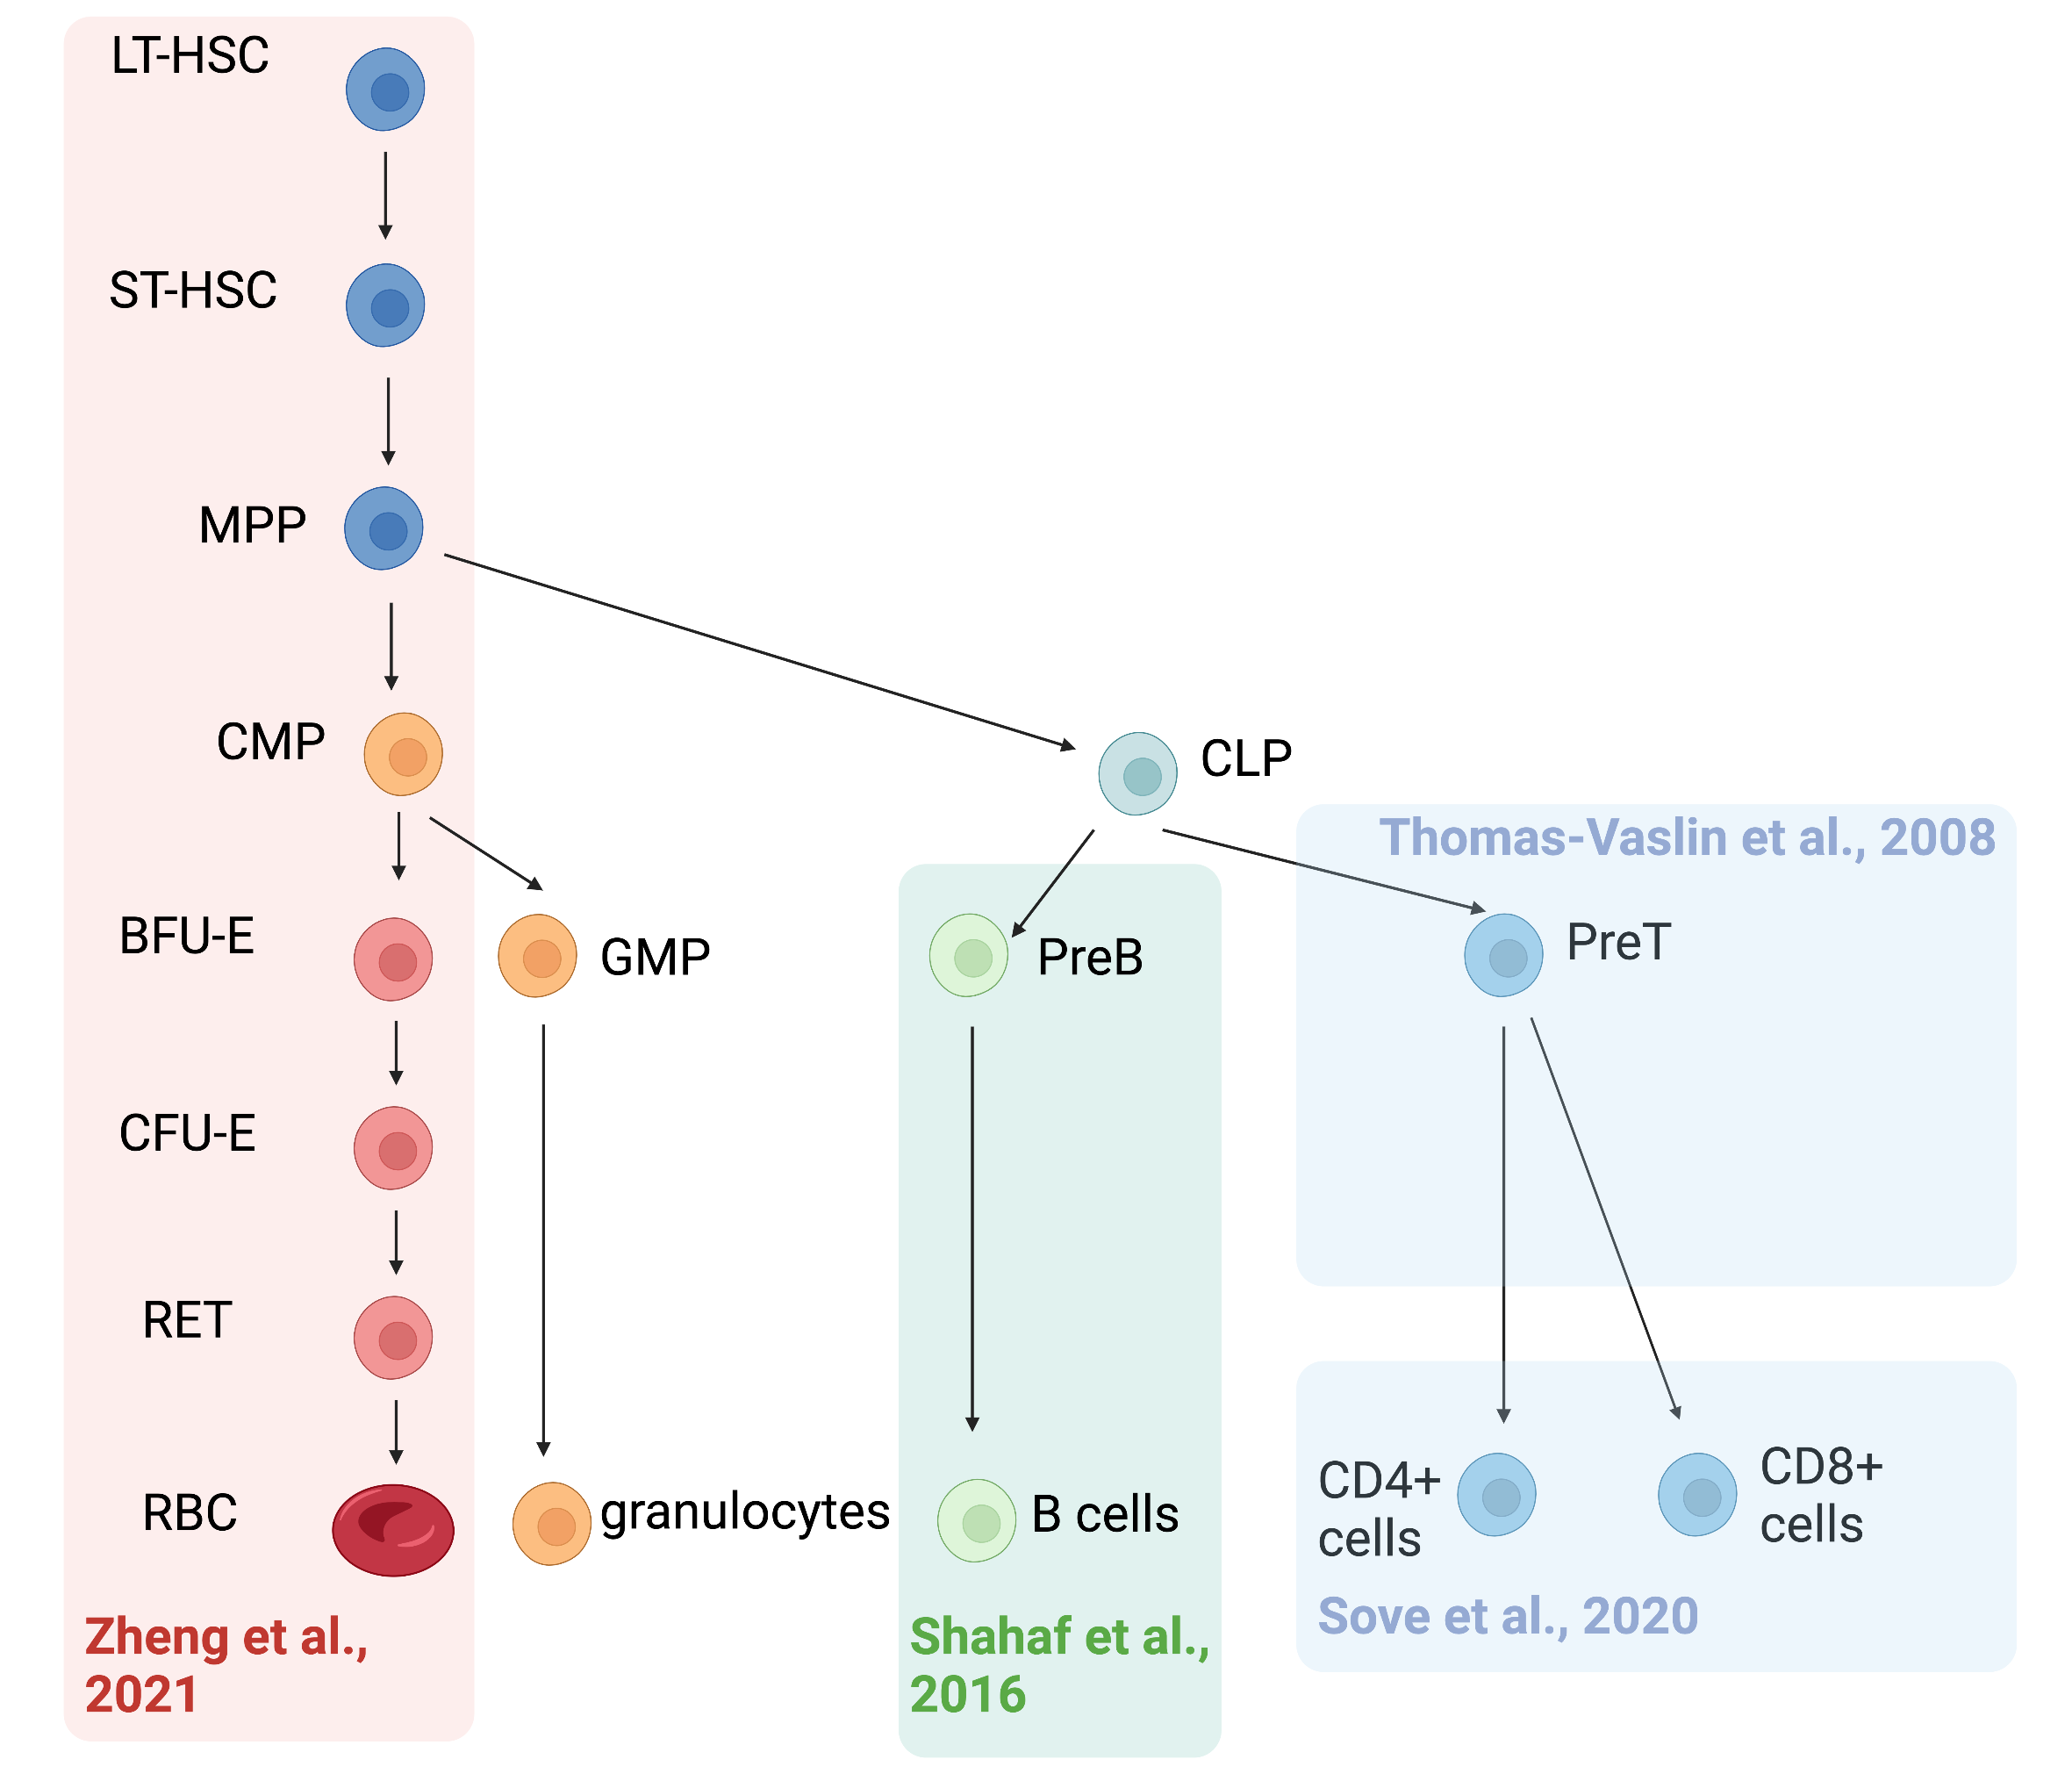
\includegraphics[width=\textwidth]{../img/Diagram_integration}

}
%%%%%%%%%%%%%%%%%%%%%%%%%%%%%%%%%%%%%%%%%%%%%%%%%%%%%%%%%%%%%%%%%%%%%%%%%%%%%%%%

\headerbox{Methods}{name=methods,column=0,below=abstract}{

% Replace this text with your Methods
We developed an integrated model that depicts the differentiation of hematopoietic stem cells (HSCs) into erythrocytes, lymphocytes, and granulocytes. The model was built incrementally by incorporating novel physiological-based features from literature while integrating published models [1-4].The resulting model represents multiple organs, including bone marrow, blood, thymus, and other lymphoid tissues. The model was developed using mice data before being scaled to human. 

}

%%%%%%%%%%%%%%%%%%%%%%%%%%%%%%%%%%%%%%%%%%%%%%%%%%%%%%%%%%%%%%%%%%%%%%%%%%%%%%%%

\headerbox{References}{name=references,column=0,below=methods}{
\footnotesize
[1] Zheng, Bo, et al. "A systems pharmacology model for gene therapy in sickle cell disease." CPT: Pharmacometrics \& Systems Pharmacology 10.7 (2021): 696-708.
[2] Shahaf, Gitit, et al. "B cell development in the bone marrow is regulated by homeostatic feedback exerted by mature B cells." Frontiers in immunology 7 (2016): 77.
[3] Thomas-Vaslin, Veronique, et al. "Comprehensive assessment and mathematical modeling of T cell population dynamics and homeostasis." The Journal of Immunology 180.4 (2008): 2240-2250.
[4] Sové, Richard J., et al. "QSP‐IO: a quantitative systems pharmacology toolbox for mechanistic multiscale modeling for Immuno‐oncology applications." CPT: pharmacometrics \& systems pharmacology 9.9 (2020): 484-497.
}
%%%%%%%%%%%%%%%%%%%%%%%%%%%%%%%%%%%%%%%%%%%%%%%%%%%%%%%%%%%%%%%%%%%%%%%%%%%%%%%%
%%%%%%%%%%%%%%%%%%%%%%%%%%%%%%%%%%%%%%%%%%%%%%%%%%%%%%%%%%%%%%%%%%%%%%%%%%%%%%%%


\headerbox{Results}{name=results,span=2,column=1,row=0}{
% Replace this text with your Results
Lorem ipsum dolor sit amet, consectetur adipiscing elit, sed do eiusmod tempor
incididunt ut labore et dolore magna aliqua. Nunc sed blandit libero volutpat
sed cras. Sit amet est placerat in egestas erat. Amet consectetur adipiscing
elit duis tristique sollicitudin nibh sit. Risus at ultrices mi tempus imperdiet
nulla. Mi bibendum neque egestas congue quisque egestas diam in arcu. Mattis
pellentesque id nibh tortor id aliquet lectus proin nibh. Netus et malesuada
fames ac turpis egestas integer eget aliquet. 



Auctor urna nunc id cursus metus
aliquam eleifend mi in. Dolor morbi non arcu risus quis. Faucibus ornare
suspendisse sed nisi lacus sed viverra tellus. Elementum curabitur vitae nunc
sed velit dignissim sodales. Aenean sed adipiscing diam donec. Amet facilisis
magna etiam tempor orci. Penatibus et magnis dis parturient montes nascetur.
Tristique et egestas quis ipsum suspendisse. Odio pellentesque diam volutpat
commodo. A scelerisque purus semper eget. Volutpat diam ut venenatis tellus in
metus.

}

%%%%%%%%%%%%%%%%%%%%%%%%%%%%%%%%%%%%%%%%%%%%%%%%%%%%%%%%%%%%%%%%%%%%%%%%%%%%%%%%


\headerbox{Conclusion}{name=conclusion,span=2,column=1,below=results}{
% Replace this text with your Conclusions
Dis parturient montes nascetur ridiculus mus mauris vitae
ultricies. Vitae elementum curabitur vitae nunc sed velit dignissim sodales.
Nunc consequat interdum varius sit amet. At elementum eu facilisis sed odio
morbi quis commodo odio. Ac turpis egestas sed tempus urna et pharetra. Quis
hendrerit dolor magna eget est lorem ipsum dolor sit. Vestibulum rhoncus est
pellentesque elit.
}

\end{poster}
\end{document}
